\scanpage{24}
% letterhead
\begin{center}
I N S T I T U T\\
DES HAUTES ÉTUDES SCIENTIFIQUES\\
\rule{1cm}{0.4pt}
\end{center}

\handwritten{SGA 4 $\overline{\text{\uline{\unsure{VII|VI}}}}$\quad p. 20}

\handwritten{\uline{Ajouter} 5.6. \textcircled{a} $\tilde{X}_{\mathrm{et}}$ est \inserted{algébrique\inserted{(ref)}, \unsure{d.|de} torsion,} localement cohérent\inserted{(ref)}. Il est cohérent \deleted{\illegible{1}}\inserted{(ref)} (\unsure{resp.} quasi-séparé\inserted{(ref)}) \deleted{\illegible{1}} \unsure{sss|ssi} le schéma $X$ est \deleted{\unsure{quasi-cpt}} cohérent i.e. qu. cpt qu. sép (resp. quasi-séparé). \deleted{\illegible{1}}}

\handwritten{\textcircled{b} Soit $(X_i)_{i\in I}$ système projectif filtrant à morphismes de transition affines, $X=\varprojlim_i X_i$ (EGA \uline{IV} 8);}

\handwritten{\unsure{Âlors|Alors}}
\[
\handwritten{\tilde{X}_{\mathrm{et}}\simeq\underset{\longleftarrow}{\mathrm{limtop}}\,\tilde{X}_i.}
\]

\handwritten{En déduire pour 5.7.}

\margin{\handwritten{\uline{Cor.} 5.6.1. $X'\in\mathrm{Ob}\,\unsure{X_{\mathrm{et}}|\tilde{X}_{\mathrm{et}}}$ est \deleted{\unsure{cohérent}} \inserted{\textcircled{\scriptsize\unsure{qu.-cpt}}} (\unsure{qu. sép}) dans $X_{\mathrm{et}}$ sss $X'$ est \deleted{\illegible{1}}. \inserted{\textcircled{\scriptsize\unsure{resp. coh}}}}}
\figure{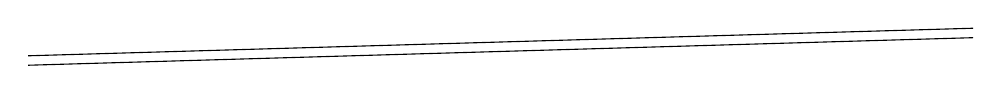
\begin{tikzpicture}\draw (0,0)--(12,0.35);\draw (0,-0.12)--(12,0.23);\end{tikzpicture}}

\handwritten{SGA 4 $\overline{\text{\uline{IX}}}$\quad p. 42\qquad note \uline{pour} la p. 8}
\figure{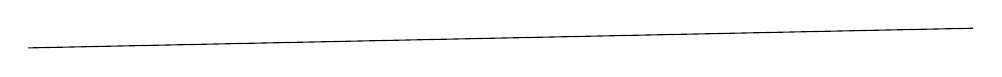
\begin{tikzpicture}\draw (0,0)--(12,0.25);\end{tikzpicture}}

\handwritten{$\overline{\text{\uline{VII}}}$\quad 2.1 c)\qquad (p. 9)\quad \uline{corriger}}
% archive sheet number: 23
